\documentclass{beamer}
\usetheme{Boadilla}
\usecolortheme{dolphin}
\usepackage{amsmath}
\usepackage{graphicx}
\usepackage{hyperref}
\graphicspath{{figs/}}

\title[4 years of GANs]{4 Years of Generative Adversarial Networks (GANs)}
\author{Lu Lu}
\institute[Crunch]{Crunch Seminar}
\date{Chinese New Year 2018}
\logo{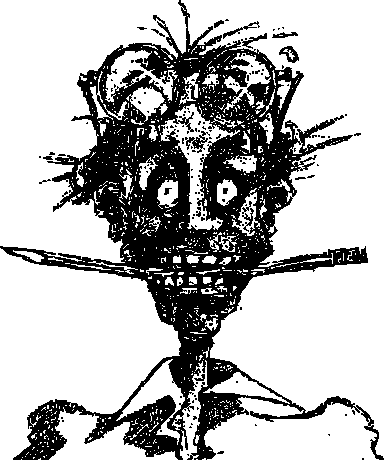
\includegraphics[height=1cm]{crunchOFF.pdf}
\includegraphics[height=1cm]{fuOFF.png}}

\begin{document}

\frame{\titlepage}

\begin{frame}
\frametitle{Best Wishes for the Year of the Dog}
\begin{figure}
  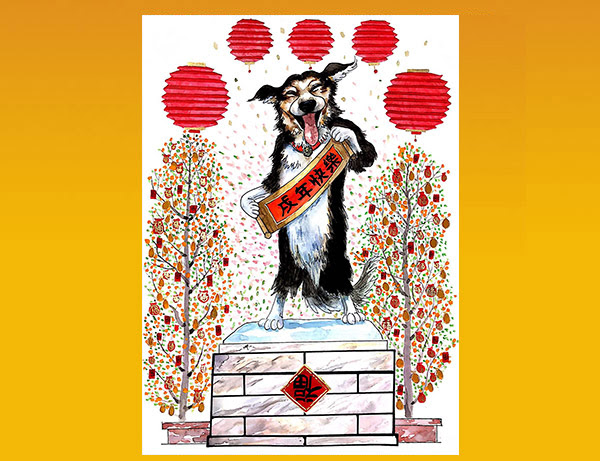
\includegraphics[height=.85\textheight]{happy_new_year.jpg}
\end{figure}
\end{frame}

\begin{frame}
\frametitle{Overview}
\tableofcontents
\end{frame}

\begin{frame}
\frametitle{Do Not Be Afraid of GANs.}
\begin{figure}
  
\includegraphics[width=.8\textwidth]{AI_simple.png}
\end{figure}
\hfill By Brandon Wirtz (CEO and Founder at Recognant), Feb 15, 2018\\
\begin{itemize}
\item ... 99\% of these things are completely stupid...
\item \textbf{So you built a neural network from scratch… And it runs on a phone…} \\
Great. So you converted 11 lines of python that would fit on a t-shirt... You have mastered what a cross compiler can do in 3 seconds.
\end{itemize}
What about GANs? 3\%.
\end{frame}

\section{What is ``adversarial''?}

\begin{frame}
\frametitle{Overview}
\tableofcontents[currentsection]
\end{frame}

\begin{frame}
\frametitle{What Is Adversarial?}
Evolve with competition
\begin{figure}
  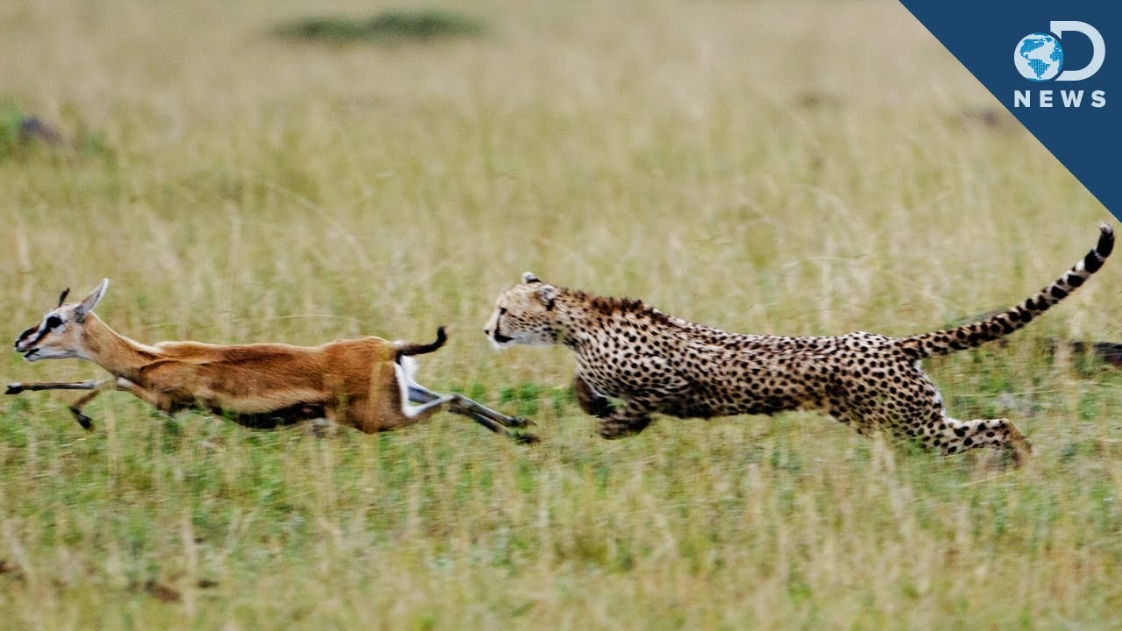
\includegraphics[height=.45\textheight]{leopard_deer.png}
\end{figure}
Deer-leopard minimax game
$$\min_{\text{leopard}} \max_{\text{deer}} V(\text{deer}, \text{leopard}) = \text{distance between deer and leopard}$$
What Doesn't Kill You Makes You Stronger!
\end{frame}

\begin{frame}
\frametitle{What Is Adversarial?}
\begin{figure}
  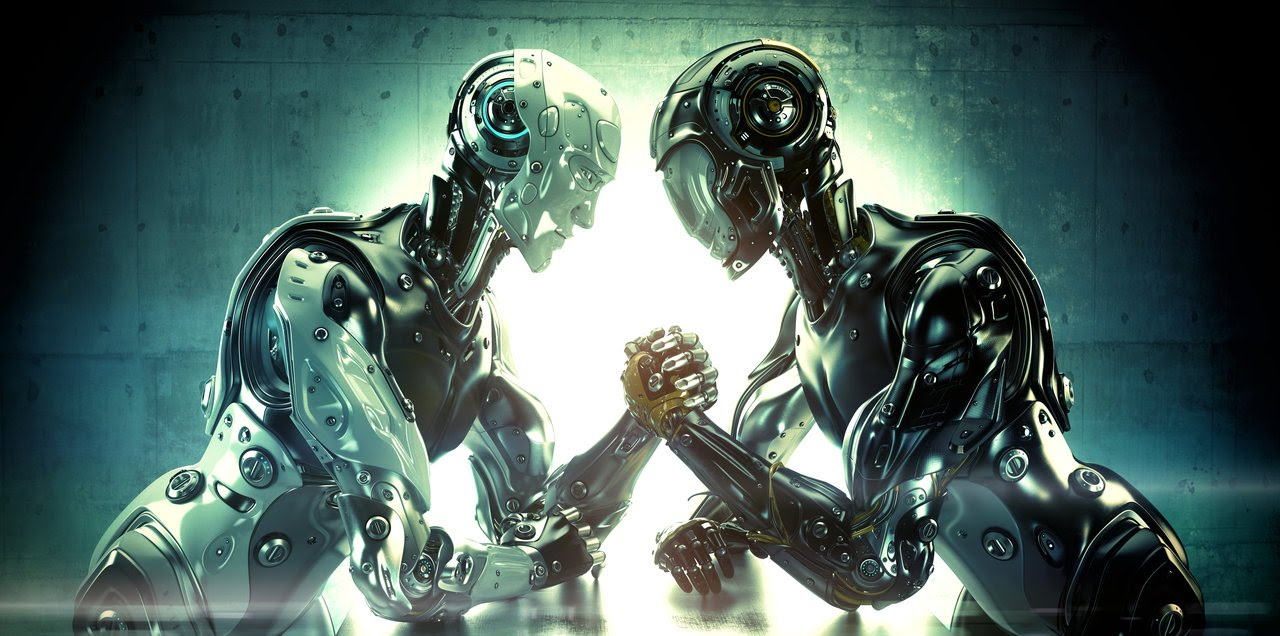
\includegraphics[height=.6\textheight]{robotic_arm_wrestling.jpg}
\end{figure}
\begin{itemize}
  % \item Adversarial examples
  \item Generative adversarial networks (GANs)
\end{itemize}
\end{frame}

\section{Generative adversarial networks (GANs)}
\subsection{Vanilla GAN}

\begin{frame}
\frametitle{Overview}
\tableofcontents[currentsection,currentsubsection]
Since 2014,
\begin{figure}
  
\includegraphics[width=\textwidth]{GAN_articles.png} \\
  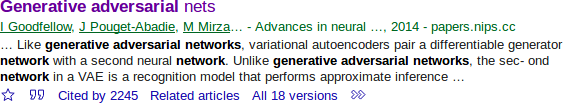
\includegraphics[width=.8\textwidth]{GAN_citation.png}
\end{figure}
\end{frame}

\begin{frame}
\frametitle{Vanilla GAN}
\begin{itemize}
\item Generator G: capture the data distribution (make realistic images)
\item Discriminator D: estimate the \textcolor{red}{probability} that a sample came from the training data rather than G (tell real and fake images apart)
\end{itemize}
\begin{figure}
  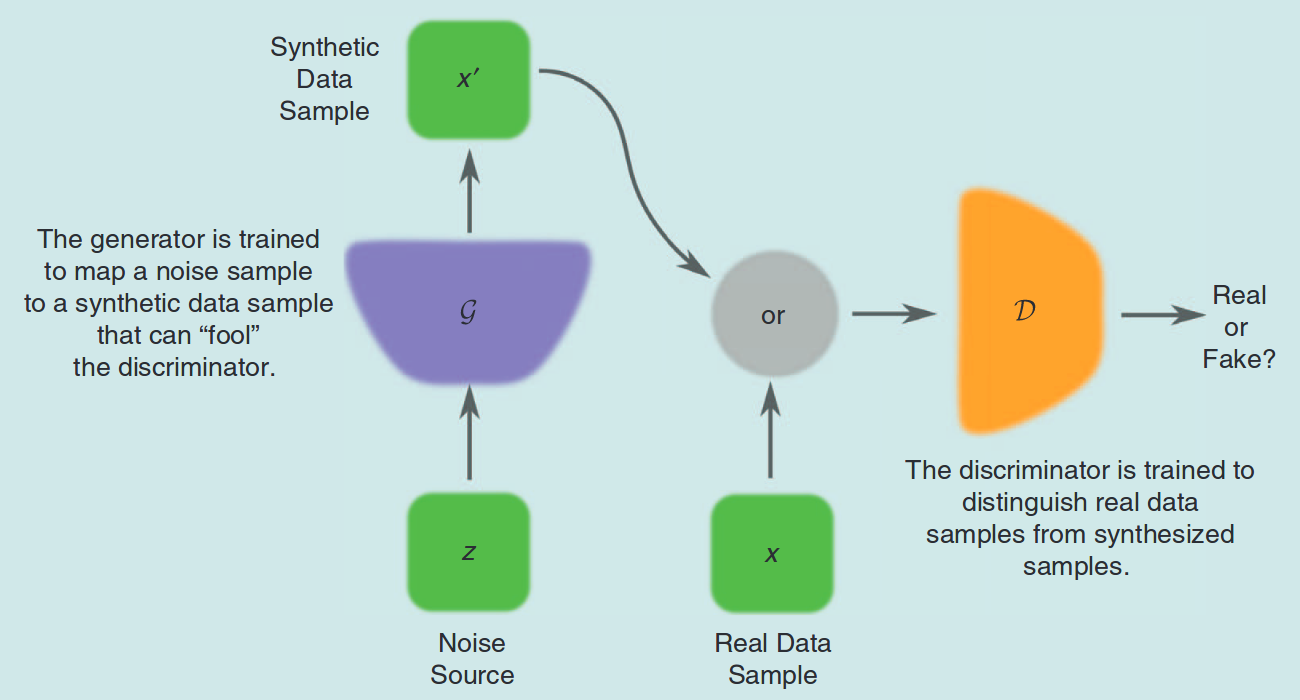
\includegraphics[height=.6\textheight]{GAN.png}
\end{figure}
\end{frame}

\begin{frame}
\frametitle{Vanilla GAN}
\begin{itemize}
  \item $p_{\mathbf{z}}(\mathbf{z})$: input noise
  \item $p_{\text{data}}(\mathbf{x})$: real data's distribution
  \item $p_g(\mathbf{x})$: generator's distribution of $G(\mathbf{z})$
\end{itemize}
Two-player minimax game
$$\min_G \max_D V(D, G) = \mathbb{E}_{\mathbf{x} \sim p_{\text{data}}(\mathbf{x})}[\log D(\mathbf{x})] + \mathbb{E}_{\mathbf{z} \sim p_{\mathbf{z}}(\mathbf{z})}[\log (1-D(G(\mathbf{z})))]$$
\begin{figure}
  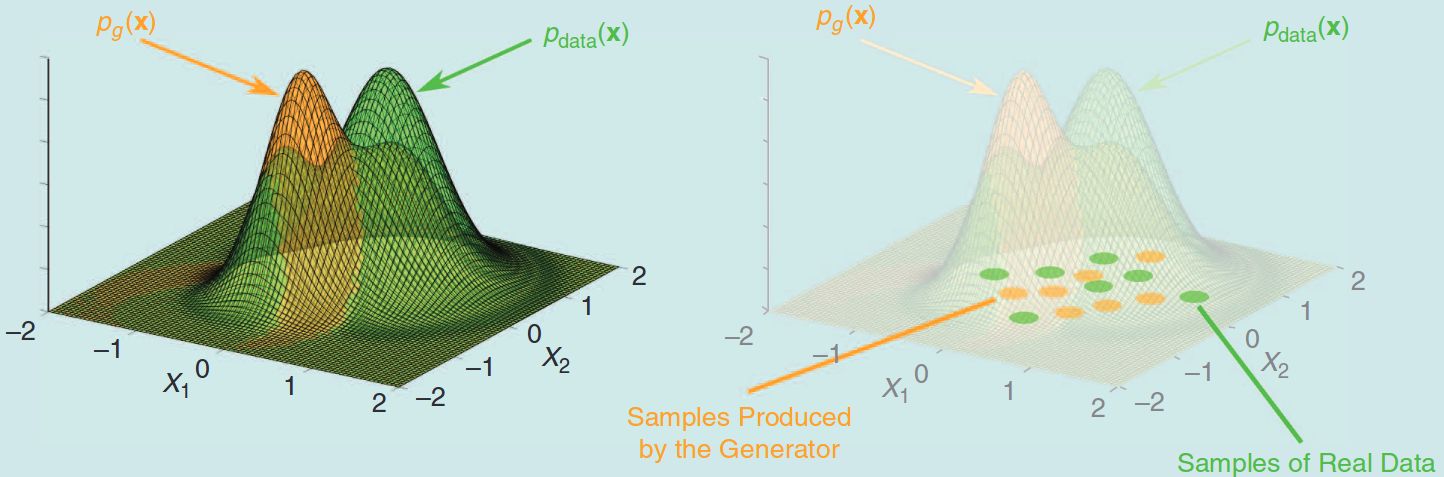
\includegraphics[height=.4\textheight]{GAN_distribution.png}
\end{figure}
\end{frame}

\begin{frame}
\frametitle{Vanilla GAN}
Main loop of GAN training
\begin{figure}
  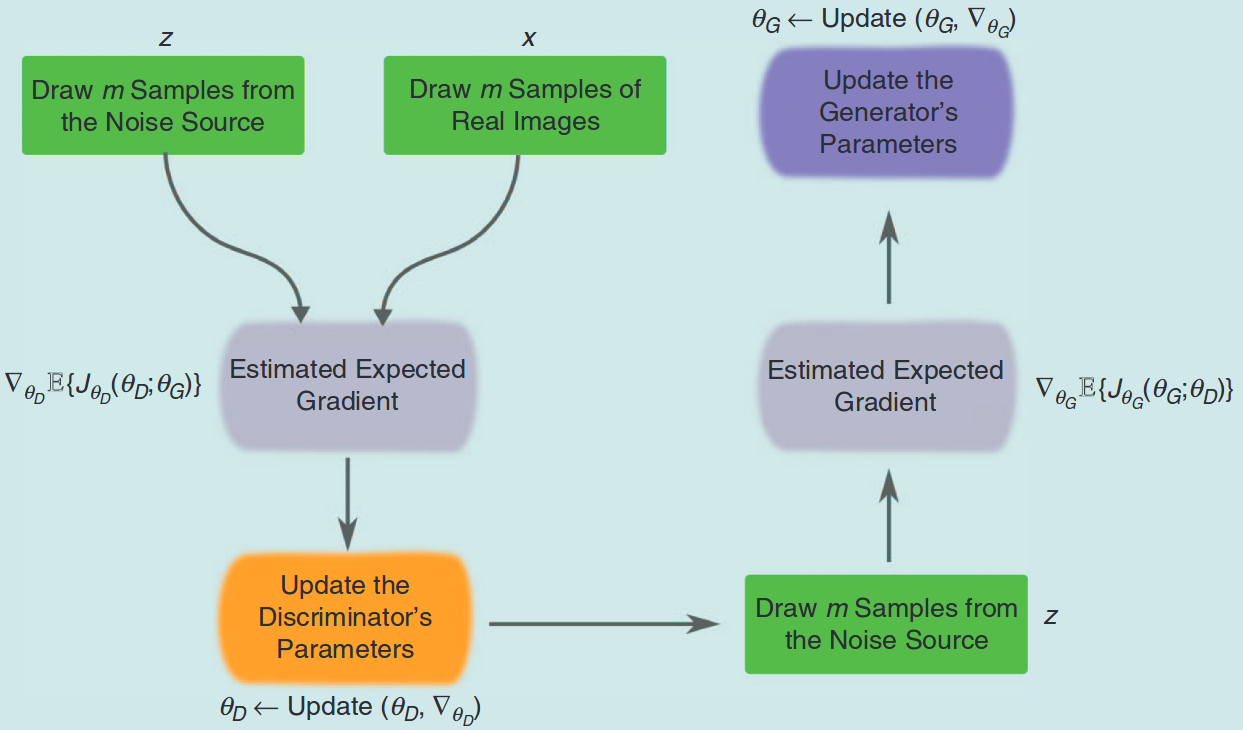
\includegraphics[height=.7\textheight]{GAN_training.png}
\end{figure}
\end{frame}

\begin{frame}
\frametitle{Vanilla GAN}
\begin{figure}
  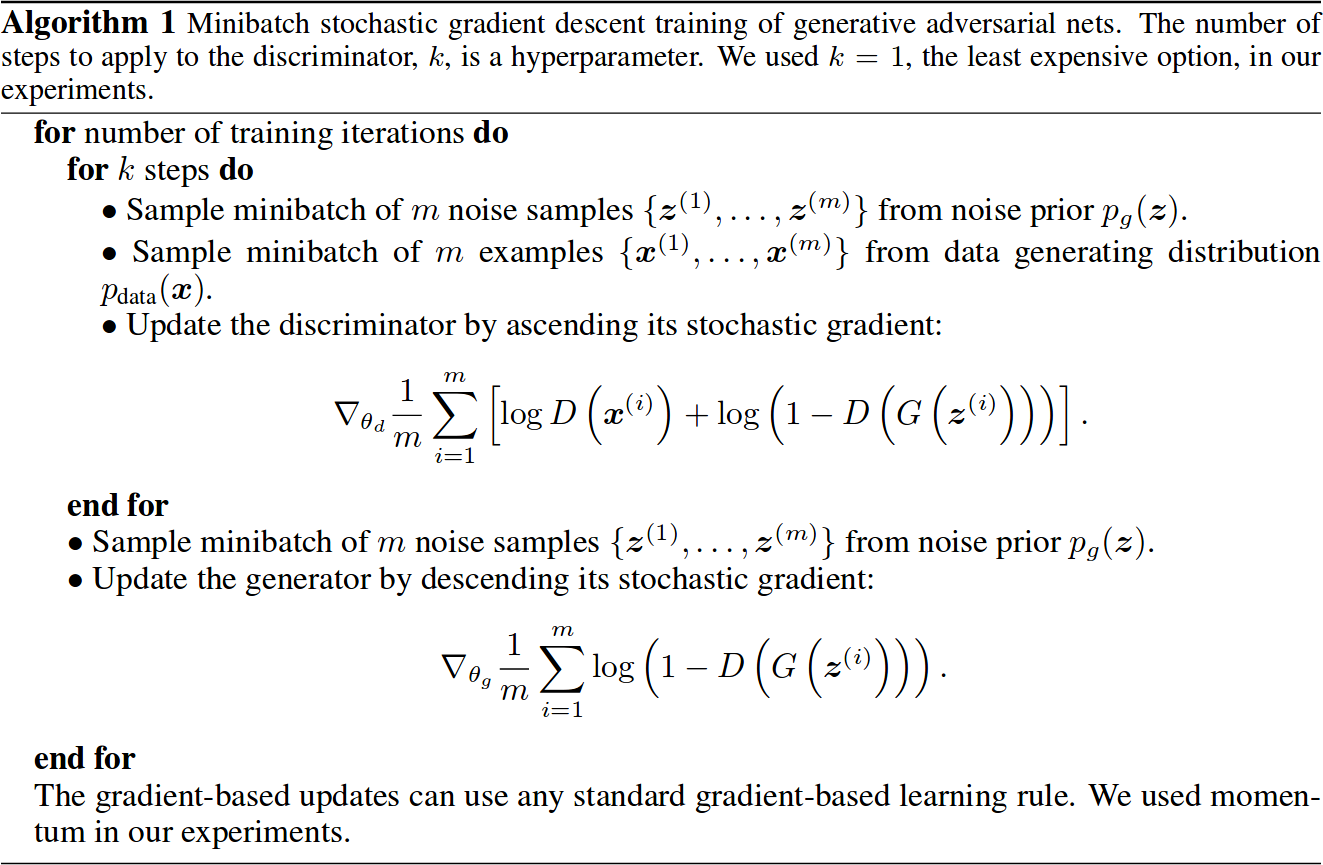
\includegraphics[height=.8\textheight]{GAN_algorithm.png}
\end{figure}
\end{frame}

\begin{frame}
\frametitle{Vanilla GAN}
\begin{figure}
  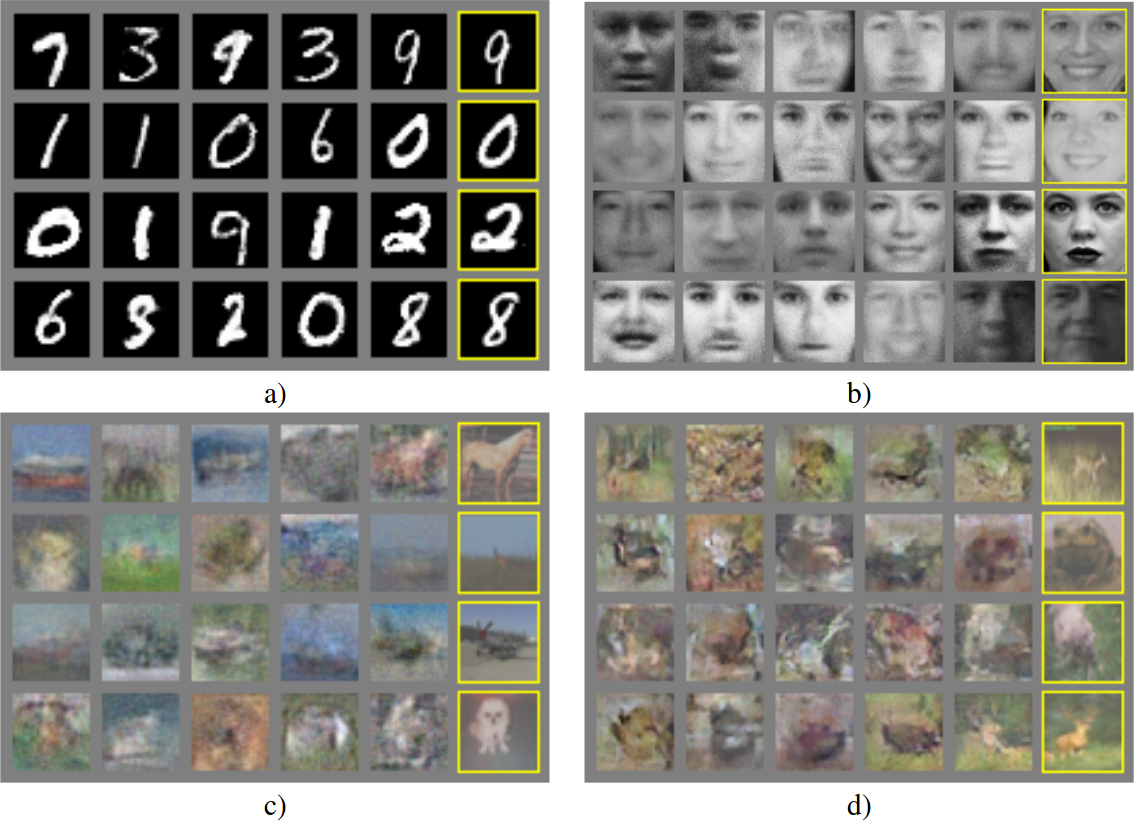
\includegraphics[height=.5\textheight]{GAN_samples.png}
\end{figure}
Difficult to train \cite{Salimans2016, Arjovsky2017a}
\begin{itemize}
  \item Vanishing gradients
  \item Instability
  \item Model collapse
  \item ...
\end{itemize}
\end{frame}

\begin{frame}
\frametitle{Improvements}
17 tips to make GANs work (\url{https://github.com/soumith/ganhacks})
\begin{itemize}
\item Use a spherical $\mathbf{z}$
\item Batch normalization \cite{Ioffe2015}
\item ...
\end{itemize}
GAN variants ($>100$)
\begin{itemize}
  % \item Laplacian pyramid GAN (LAPGAN) \cite{Denton2015}
  \item Deep convolutional GAN (DCGAN) \cite{Radford2015}
  \item Conditional GAN \cite{Mirza2014}
  \item Adversarially learned inference (ALI) \cite{Dumoulin2016}
  % \item Bidirectional GAN (BiGAN)
  \item Adversarial autoencoder (AAE) \cite{Makhzani2015}
  % \item Adversarial variational bayes (AVB) \cite{Mescheder2017}
  \item Energy-based GAN (EBGAN) \cite{Zhao2016}
  \item \textcolor{red}{Wasserstein GAN (WGAN)} \cite{Arjovsky2017b}
  \item Boundary equilibrium GAN (BEGAN) \cite{Berthelot2017}
  \item Bayesian GAN \cite{Saatchi2017}
  \item ...
\end{itemize}
\end{frame}

\subsection{WGAN}

\begin{frame}
\frametitle{Overview}
\tableofcontents[currentsection,currentsubsection]
\end{frame}

\begin{frame}
\frametitle{WGAN}
Recall GAN
$$\min_G \max_D V(D, G) = \mathbb{E}_{\mathbf{x} \sim p_{\text{data}}(\mathbf{x})}[\log D(\mathbf{x})] + \mathbb{E}_{\mathbf{z} \sim p_{\mathbf{z}}(\mathbf{z})}[\log (1-D(G(\mathbf{z})))]$$
Earth-Mover (EM) distance or Wasserstein-1 \cite{Monge1781}
$$W(\mathbb{P}_r, \mathbb{P}_g) = \inf_{\gamma \in \Pi(\mathbb{P}_r, \mathbb{P}_g)} \mathbb{E}_{(x,y) \sim \gamma}[||x-y||]$$
By Kantorovich-Rubinstein duality \cite{Villani2008},
$$W(\mathbb{P}_r, \mathbb{P}_{\theta}) = \sup_{||f||_L\leq 1} \mathbb{E}_{x \sim \mathbb{P}_r}[f(x)] - \mathbb{E}_{x \sim \mathbb{P}_{\theta}}[f(x)]$$
Discriminator $f_w$, generator $g_{\theta}$
$$\min_{\theta}\max_{w \in \mathcal{W}} \mathbb{E}_{x \sim \mathbb{P}_r}[f_w(x)] - \mathbb{E}_{z \sim p(z)}[f_w(g_{\theta}(z))]$$
\end{frame}

\begin{frame}
\frametitle{WGAN}
\begin{figure}
  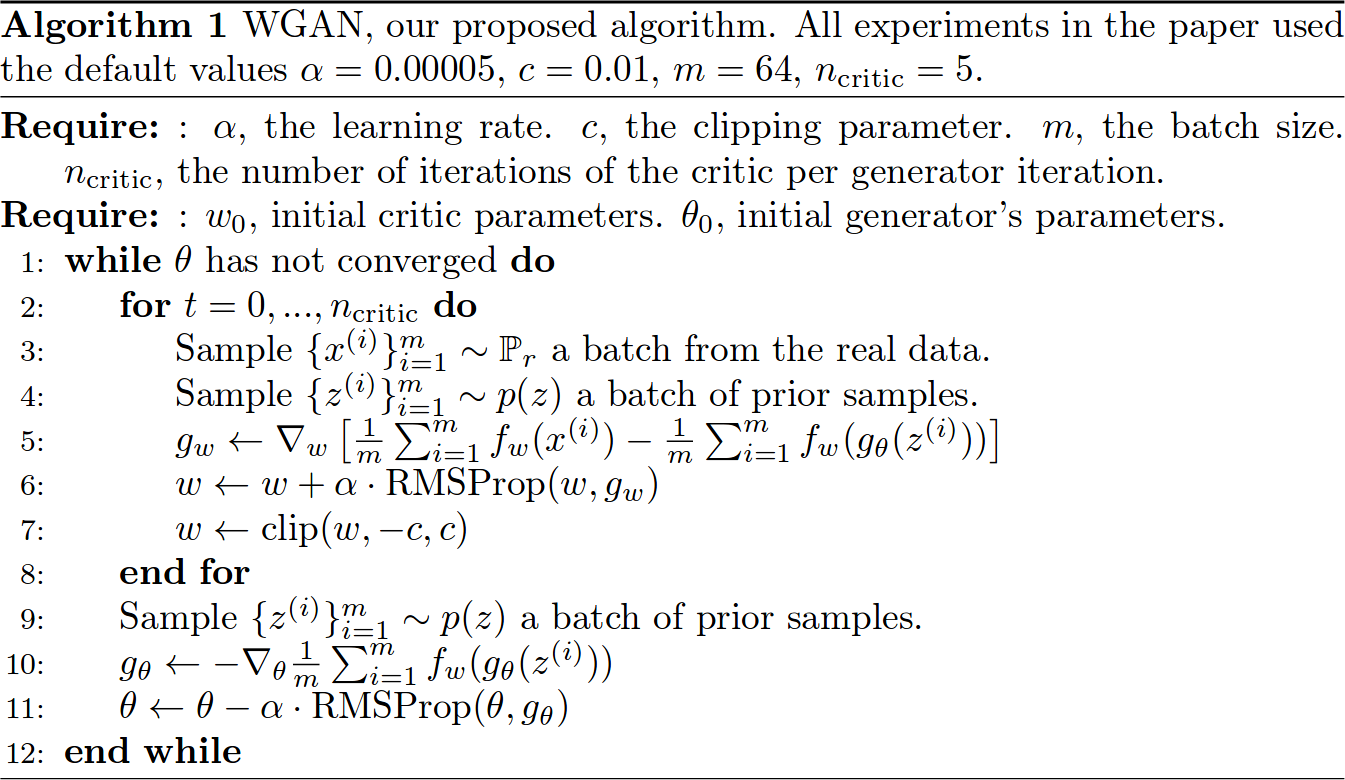
\includegraphics[height=.7\textheight]{WGAN_algorithm.png}
\end{figure}
\end{frame}

\begin{frame}
\frametitle{WGAN}
\begin{itemize}
\item Improved stability of learning
\item Get rid of mode collapse
\item Meaningful learning curves
\end{itemize}
GAN without tricks during training
\begin{figure}
  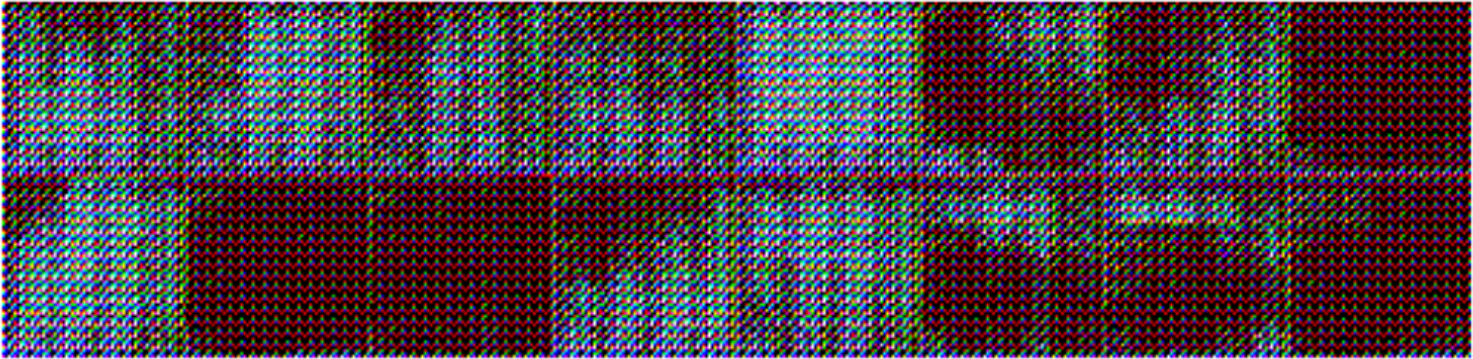
\includegraphics[height=.25\textheight]{GAN_wo_batchnorm.png}
\end{figure}
WGAN samples
\begin{figure}
  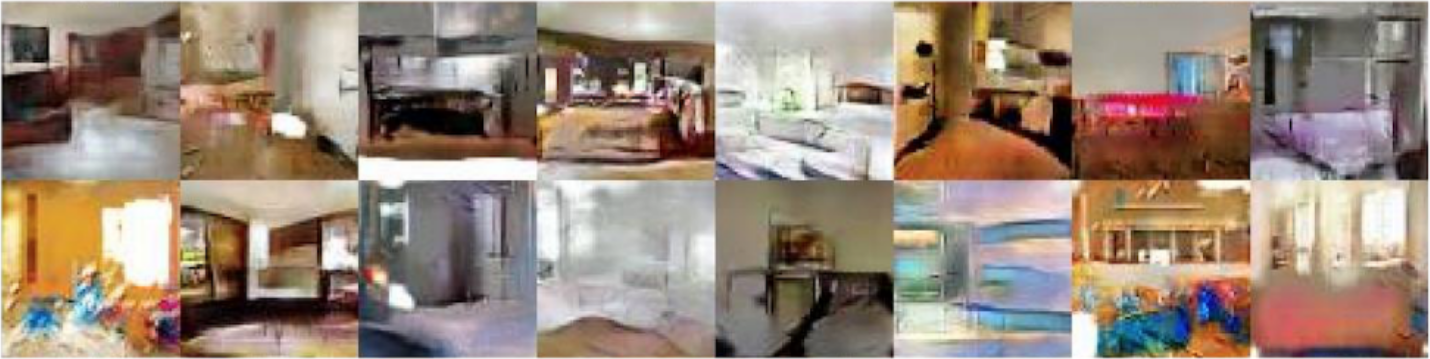
\includegraphics[height=.25\textheight]{WGAN_samples.png}
\end{figure}
\end{frame}

\section{Paper review: Daskalakis, Training GANs with optimism, 2017}

\begin{frame}
  \frametitle{Overview}
  \tableofcontents[currentsection]
\end{frame}

\begin{frame}
\frametitle{Problem of WGAN}
Limit cycling behavior in training (W)GAN
\begin{figure}
  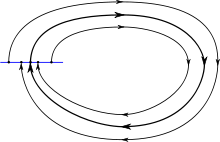
\includegraphics[height=.3\textheight]{limit_cycle.png}
\end{figure}
[\url{https://en.wikipedia.org/wiki/Limit_cycle}]
% Average does indeed equal to the true vector.
\end{frame}

\begin{frame}
\frametitle{\small{Gradient Descent (GD) vs. Optimistic Mirror Descent (OMD)}}
GD
$$w_{t+1} = w_t + \eta \cdot \nabla_{w,t}$$
$$\theta_{t+1} = \theta_t - \eta \cdot \nabla_{\theta,t}$$
OMD \cite{Rakhlin2013}: $M_{\cdot,t+1}$ is a predictor of $\nabla_{\cdot,t}$
$$w_{t+1} = w_t + \eta \cdot (\nabla_{w,t} + M_{w,t+1} - M_{w,t})$$
$$\theta_{t+1} = \theta_t - \eta \cdot (\nabla_{\theta,t} + M_{\theta,t+1} - M_{\theta,t})$$
In this paper, choose $M_{\cdot,t+1} = \nabla_{\cdot, t}$
$$w_{t+1} = w_t + \eta \cdot (2\nabla_{w,t} - \nabla_{w,t-1}) = w_t + 2\eta \cdot \nabla_{w,t} - \eta \cdot \nabla_{w,t-1}$$
$$\theta_{t+1} = \theta_t - \eta \cdot (2\nabla_{\theta,t} - \nabla_{\theta,t-1}) = \theta_t - 2\eta \cdot \nabla_{\theta,t} + \eta \cdot \nabla_{\theta,t-1})$$
\end{frame}

\begin{frame}
\frametitle{\small{Gradient Descent (GD) vs. Optimistic Mirror Descent (OMD)}}
\begin{figure}
  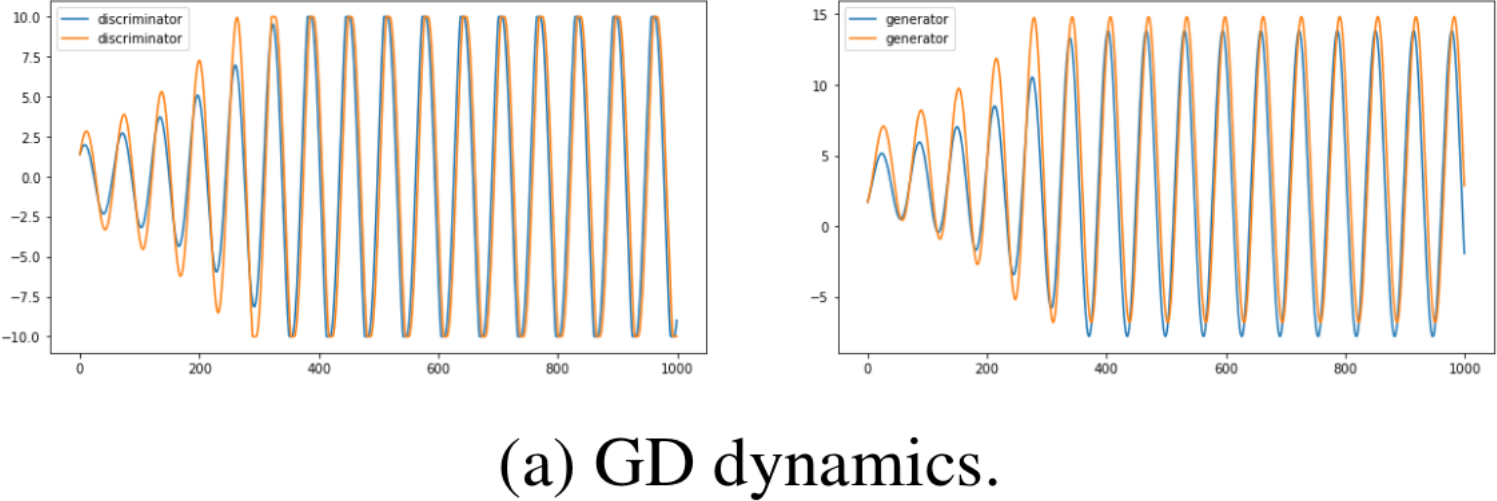
\includegraphics[width=.75\textwidth]{GD.png} \\
  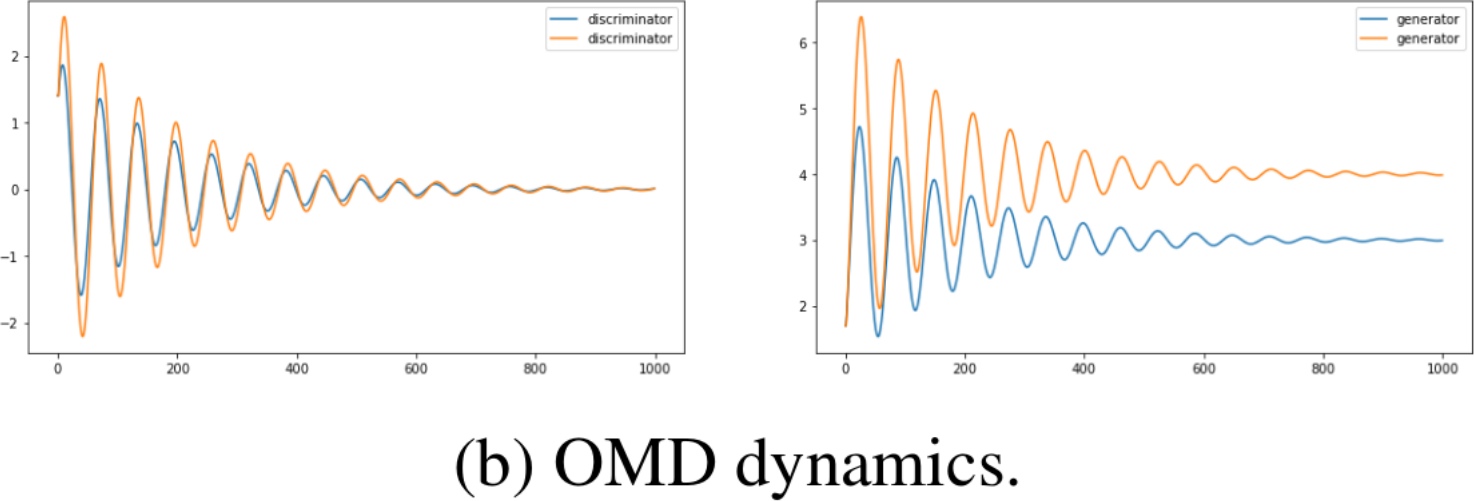
\includegraphics[width=.75\textwidth]{OMD.png}
\end{figure}
OMD dynamics converge in terms of the last iterate.
\end{frame}

\begin{frame}
\frametitle{Optimistic ADAM}
ADAM (adaptive moment estimation) \cite{Kingma2014} (6475 citations)
\begin{figure}
  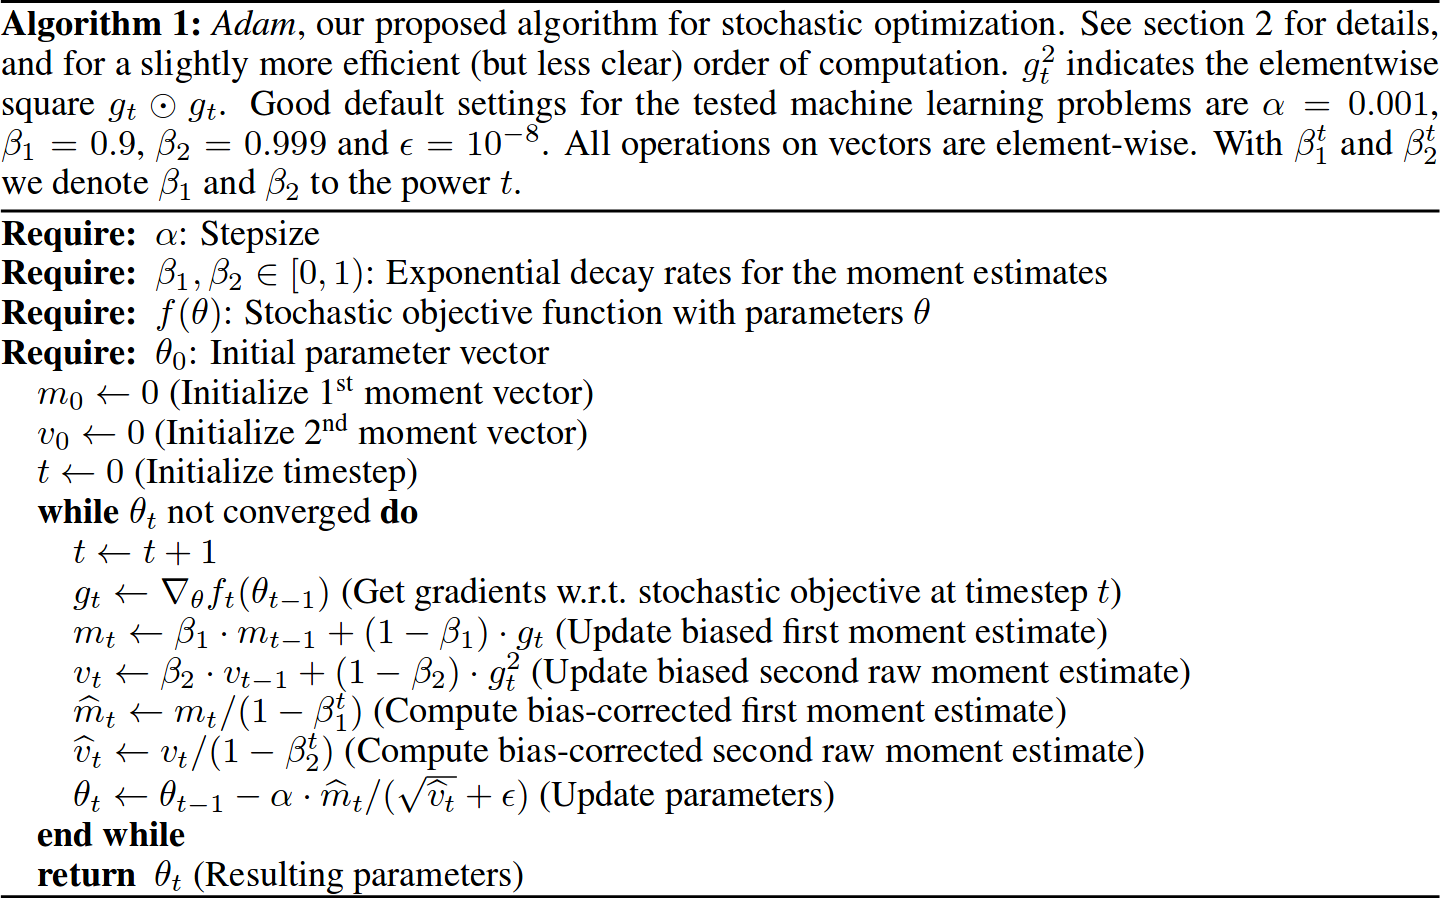
\includegraphics[width=.9\textwidth]{Adam.png}
\end{figure}
\end{frame}

\begin{frame}
\frametitle{Optimistic ADAM}
ADAM:
$$\theta_t = \theta_{t-1} - \eta \cdot \frac{\hat{m}_t}{\sqrt{\hat{v}_t} + \epsilon}$$
where $\hat{m}_t$ is first moment, $\hat{v}_t$ is second moment
\begin{figure}
  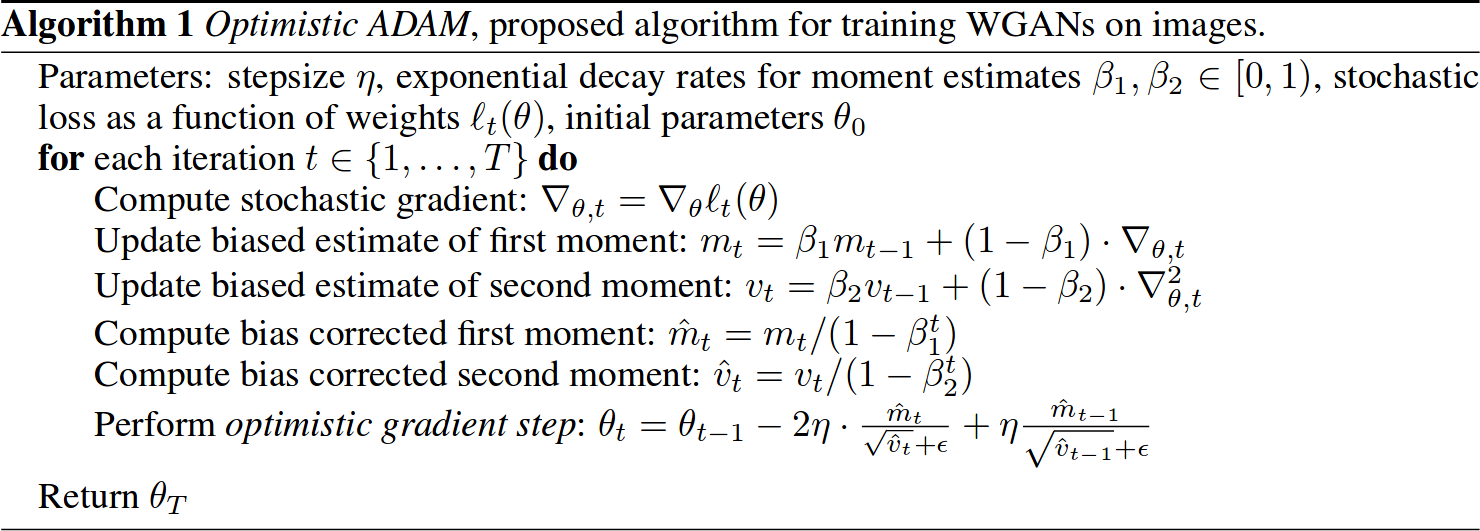
\includegraphics[width=\textwidth]{OptimisticADAM.png}
\end{figure}
\end{frame}

\begin{frame}
\frametitle{Optimistic ADAM}
\begin{figure}
  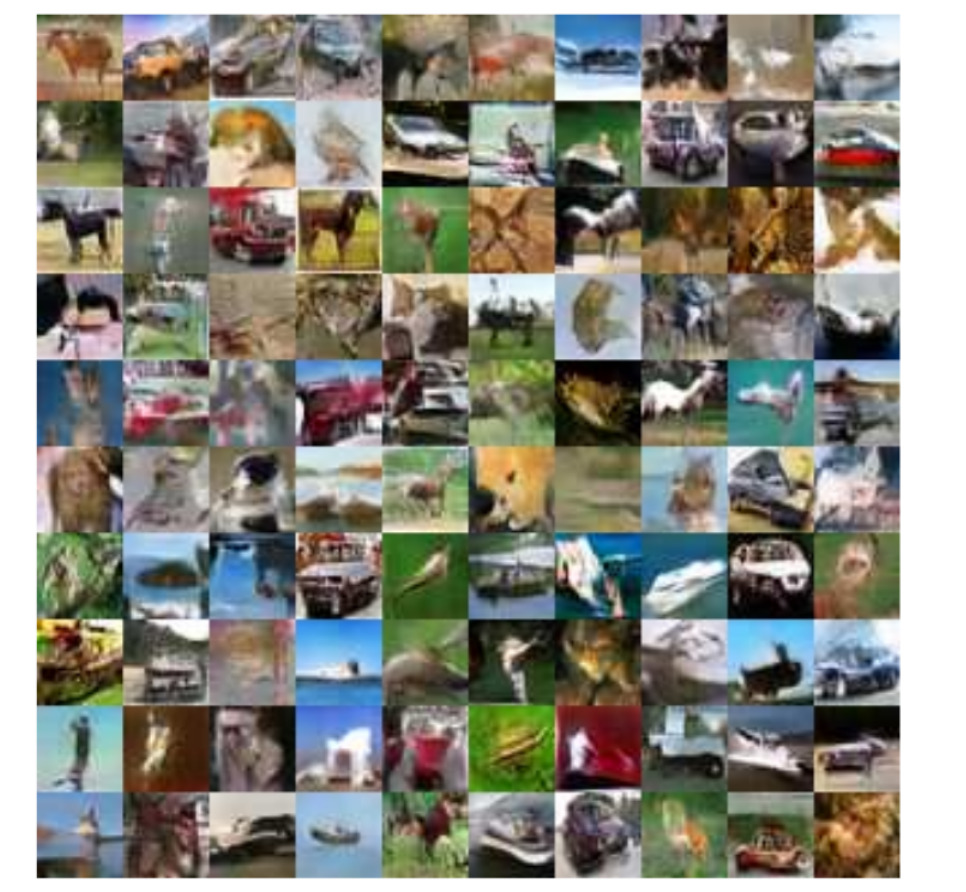
\includegraphics[width=.7\textwidth]{GAN_optimism.jpg}
\end{figure}
\end{frame}

\section{Boundary equilibrium GAN (BEGAN)}

\begin{frame}
  \frametitle{Overview}
  \tableofcontents[currentsection]
\end{frame}

\begin{frame}
\frametitle{Boundary equilibrium GAN (BEGAN)}
Samples
\begin{figure}
  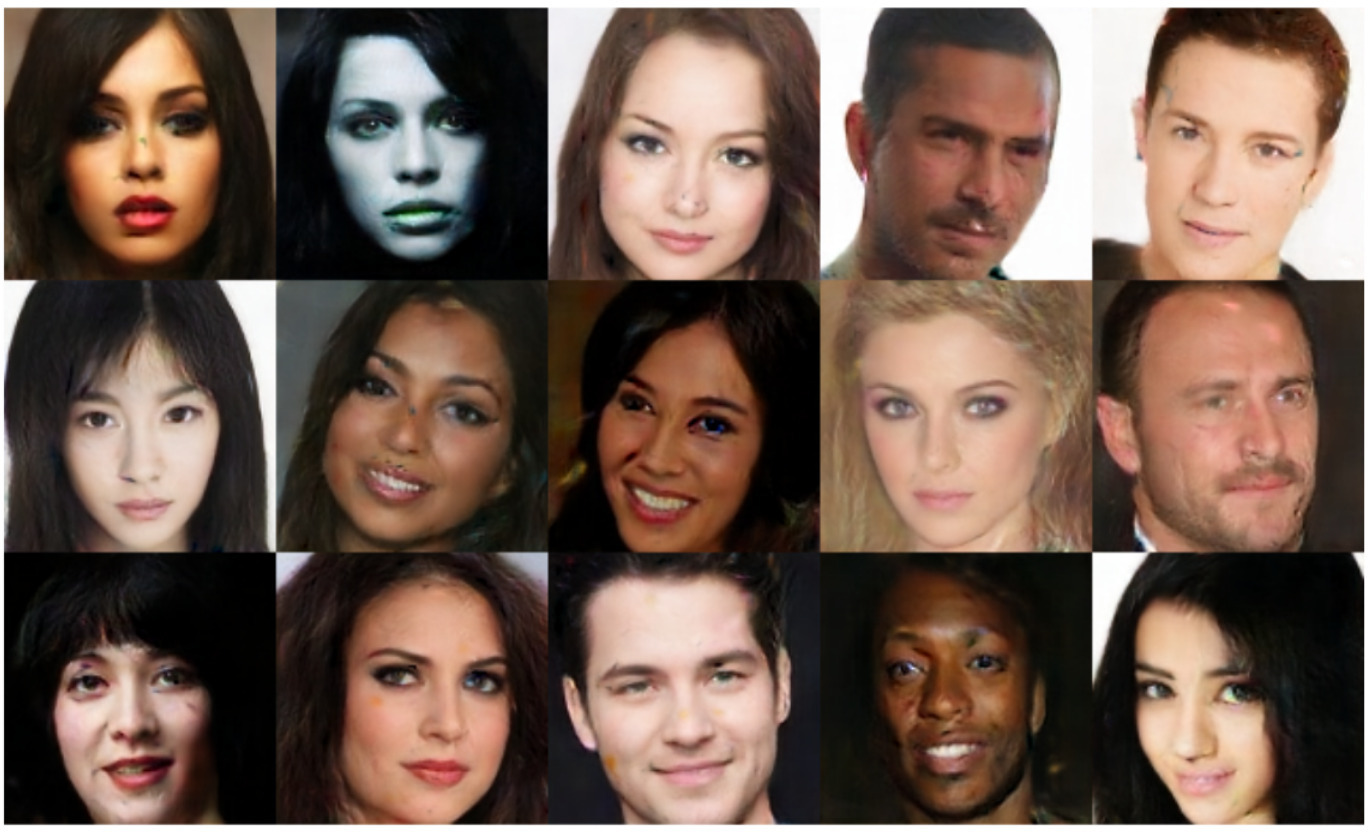
\includegraphics[height=.3\textheight]{BEGAN_samples1.jpg} \\
\end{figure}
Interpolations of real images
\begin{figure}
  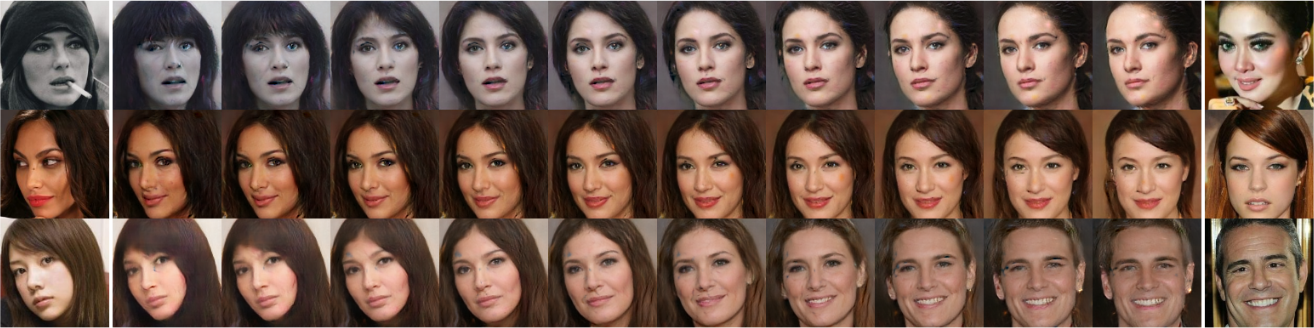
\includegraphics[height=.3\textheight]{BEGAN_samples2.png} \\
  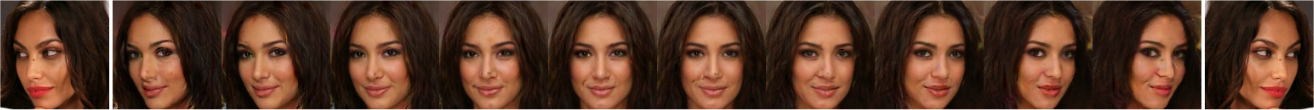
\includegraphics[height=.1\textheight]{BEGAN_samples3.png}
\end{figure}
\end{frame}

\section{Adversarial examples}

\begin{frame}
\frametitle{Overview}
\tableofcontents[currentsection]
\end{frame}

\begin{frame}
\frametitle{Adversarial Examples}
\begin{itemize}
\item Examples that are similar to examples in the true distribution, but that fool a classifier \cite{Szegedy2013}
\item A demonstration of adversarial example \cite{Goodfellow2014a}
\end{itemize}
\begin{figure}
  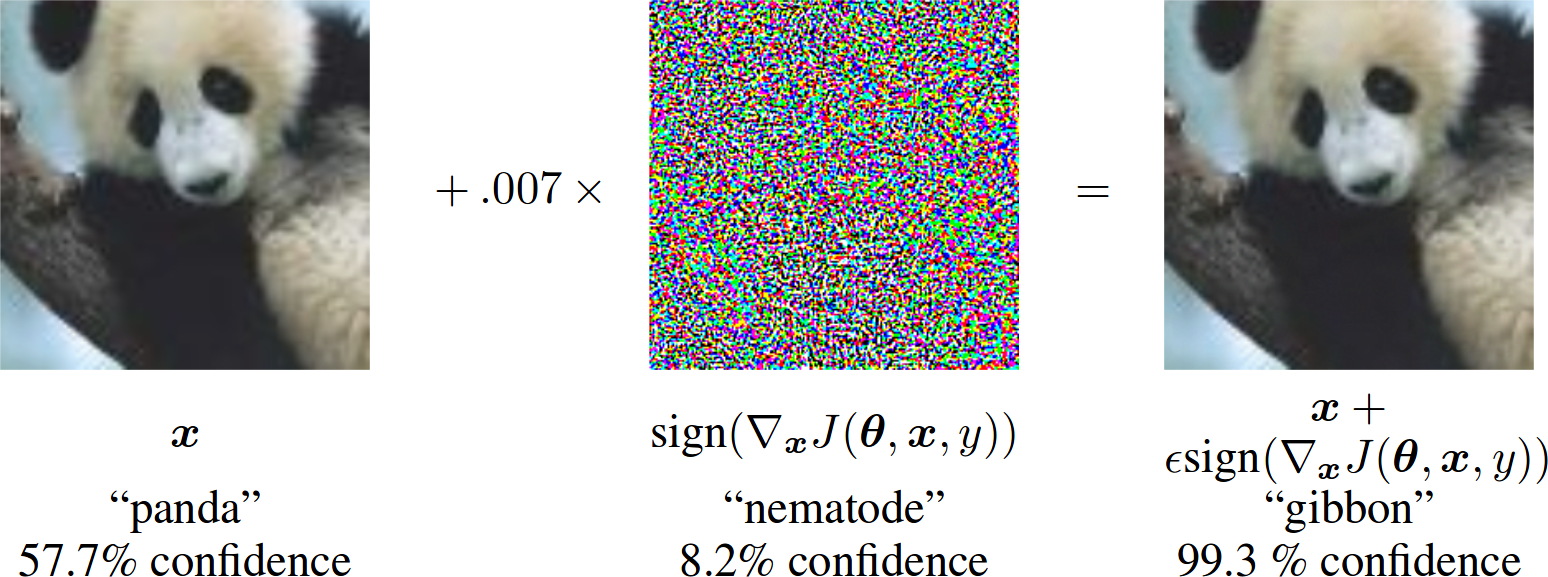
\includegraphics[width=.8\textwidth]{panda.png}
\end{figure}
Paper review: Ilyas, The Robust Manifold Defense: Adversarial Training using Generative Models, 2017.
\end{frame}

\begin{frame}
\frametitle{Adversarial Examples}
Art?
\begin{figure}
  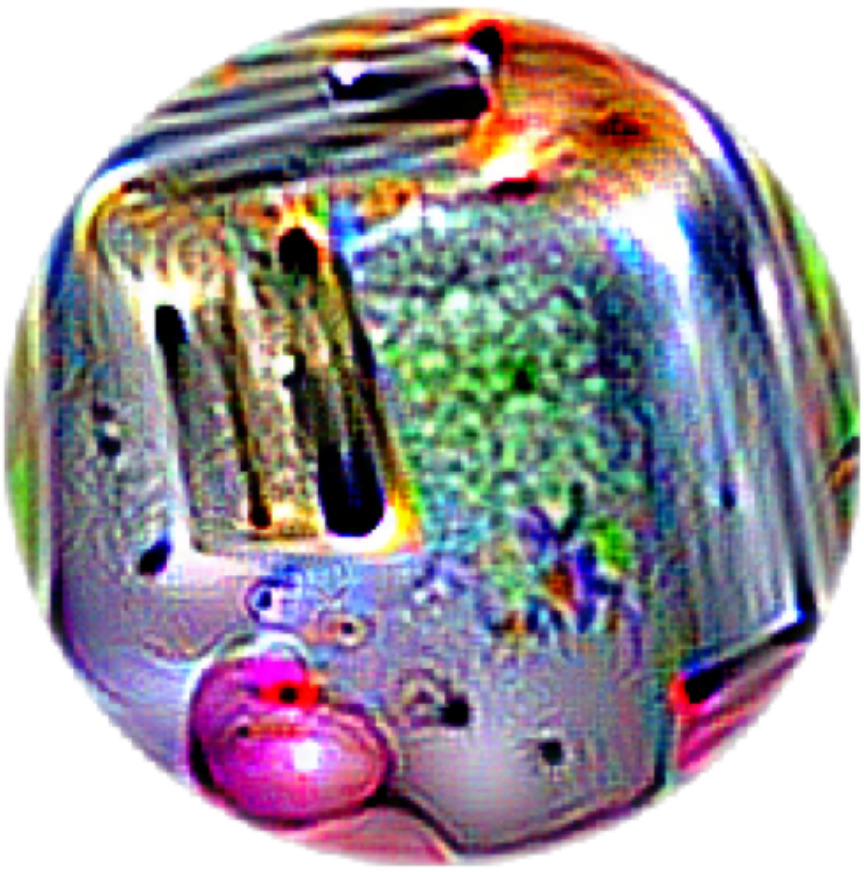
\includegraphics[height=.7\textheight]{adversarial_patch.jpg}
\end{figure}
\end{frame}

\begin{frame}
\frametitle{Adversarial Examples}
\begin{itemize}
\item Why small changes?
\item Universal, robust, targeted adversarial image patches in the real world \cite{Brown2017}
\item \url{https://youtu.be/i1sp4X57TL4}
\end{itemize}
\begin{figure}
  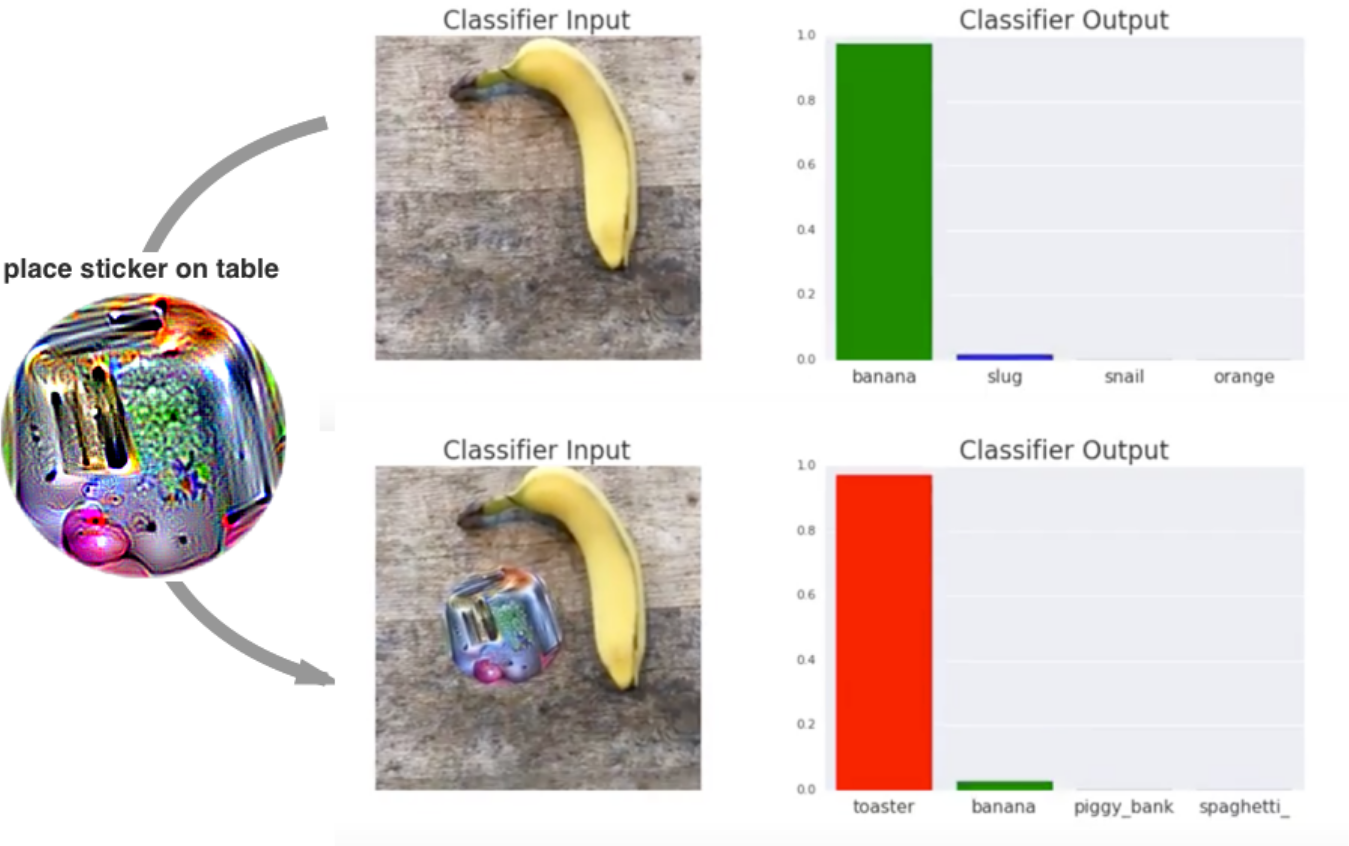
\includegraphics[width=.7\textwidth]{banana.png}
\end{figure}
\end{frame}

\begin{frame}[allowframebreaks]
\frametitle{References}
{\footnotesize
\begin{thebibliography}{99} % Beamer does not support BibTeX so references must be inserted manually as below

\bibitem[Szegedy, 2013]{Szegedy2013} Szegedy, C., Zaremba, W., Sutskever, I., Bruna, J., Erhan, D., Goodfellow, I., \& Fergus, R. (2013).
\newblock Intriguing properties of neural networks.
\newblock \emph{arXiv preprint arXiv:1312.6199}.

\bibitem[Goodfellow, 2014a]{Goodfellow2014a} Goodfellow, I. J., Shlens, J., \& Szegedy, C. (2014).
\newblock Explaining and harnessing adversarial examples.
\newblock \emph{arXiv preprint arXiv:1412.6572}.

\bibitem[Brown, 2017]{Brown2017} Brown, T. B., Mané, D., Roy, A., Abadi, M., \& Gilmer, J. (2017).
\newblock Adversarial patch.
\newblock \emph{arXiv preprint arXiv:1712.09665}.

\bibitem[Goodfellow, 2014b]{Goodfellow2014b} Goodfellow, I., Pouget-Abadie, J., Mirza, M., Xu, B., Warde-Farley, D., Ozair, S., ... \& Bengio, Y. (2014).
\newblock Generative adversarial nets.
\newblock \emph{Advances in neural information processing systems}, 2672--2680.

\bibitem[Salimans, 2016]{Salimans2016} Salimans, T., Goodfellow, I., Zaremba, W., Cheung, V., Radford, A., \& Chen, X. (2016).
\newblock Improved techniques for training gans.
\newblock \emph{Advances in Neural Information Processing Systems}, 2234--2242.

\bibitem[Arjovsky, 2017a]{Arjovsky2017a} Arjovsky, M., \& Bottou, L. (2017).
\newblock Towards principled methods for training generative adversarial networks.
\newblock \emph{arXiv preprint arXiv:1701.04862}.

\bibitem[Ioffe, 2015]{Ioffe2015} Ioffe, S., \& Szegedy, C. (2015).
\newblock Batch normalization: Accelerating deep network training by reducing internal covariate shift.
\newblock \emph{International conference on machine learning}, 448--456.

\bibitem[Denton, 2015]{Denton2015} Denton, E. L., Chintala, S., \& Fergus, R. (2015).
\newblock Deep generative image models using a laplacian pyramid of adversarial networks.
\newblock \emph{Advances in neural information processing systems}, 1486--1494.

\bibitem[Radford, 2015]{Radford2015} Radford, A., Metz, L., \& Chintala, S. (2015).
\newblock Unsupervised representation learning with deep convolutional generative adversarial networks.
\newblock \emph{arXiv preprint arXiv:1511.06434}.

\bibitem[Mirza, 2014]{Mirza2014} Mirza, M., \& Osindero, S. (2014).
\newblock Conditional generative adversarial nets.
\newblock \emph{arXiv preprint arXiv:1411.1784}.

\bibitem[Dumoulin, 2016]{Dumoulin2016} Dumoulin, V., Belghazi, I., Poole, B., Lamb, A., Arjovsky, M., Mastropietro, O., \& Courville, A. (2016).
\newblock Adversarially learned inference.
\newblock \emph{arXiv preprint arXiv:1606.00704}.

\bibitem[Makhzani, 2015]{Makhzani2015} Makhzani, A., Shlens, J., Jaitly, N., Goodfellow, I., \& Frey, B. (2015).
\newblock Adversarial autoencoders.
\newblock \emph{arXiv preprint arXiv:1511.05644}.

\bibitem[Mescheder, 2017]{Mescheder2017} Mescheder, L., Nowozin, S., \& Geiger, A. (2017).
\newblock Adversarial variational bayes: Unifying variational autoencoders and generative adversarial networks.
\newblock \emph{arXiv preprint arXiv:1701.04722}.

\bibitem[Zhao, 2016]{Zhao2016} Zhao, J., Mathieu, M., \& LeCun, Y. (2016).
\newblock Energy-based generative adversarial network.
\newblock \emph{arXiv preprint arXiv:1609.03126}.

\bibitem[Arjovsky, 2017b]{Arjovsky2017b} Arjovsky, M., Chintala, S., \& Bottou, L. (2017).
\newblock Wasserstein gan.
\newblock \emph{arXiv preprint arXiv:1701.07875}.

\bibitem[Berthelot, 2017]{Berthelot2017} Berthelot, D., Schumm, T., \& Metz, L. (2017).
\newblock Began: Boundary equilibrium generative adversarial networks.
\newblock \emph{arXiv preprint arXiv:1703.10717}.

\bibitem[Saatchi, 2017]{Saatchi2017} Saatchi, Y., \& Wilson, A. G. (2017).
\newblock Bayesian GAN.
\newblock \emph{Advances in Neural Information Processing Systems}, 3625--3634.

\bibitem[Monge, 1781]{Monge1781} avec les Memoires de Mathematique et de Physique. 1781.
\newblock Memoire sur la theorie des deblais et des remblais.
\newblock \emph{Histoire de l'Academie Royale des Science}, Annee 1781.

\bibitem[Villani, 2008]{Villani2008} Villani, C. (2008).
\newblock Optimal transport: old and new.
\newblock \emph{Springer Science \& Business Media}.

\bibitem[Rakhlin, 2013]{Rakhlin2013} Rakhlin, S., \& Sridharan, K. (2013).
\newblock Optimization, learning, and games with predictable sequences.
\newblock \emph{Advances in Neural Information Processing Systems}, 3066--3074.

\bibitem[Kingma, 2014]{Kingma2014} Kingma, D. P., \& Ba, J. (2014).
\newblock Adam: A method for stochastic optimization.
\newblock \emph{arXiv preprint arXiv:1412.6980}.

\end{thebibliography}}
\Huge{\centerline{Thank you!}}
\end{frame}

\end{document}
